

\documentclass{beamer}
\setbeamertemplate{caption}{\insertcaption}

\mode<presentation> {
	
	% The Beamer class comes with several default slide themes
	%, which changes the colors and layouts of slides. Below is a list
	% of all the themes, uncomment each, in turn, to see what they look like.
	
	%\usetheme{default}
	%\usetheme{AnnArbor}
	%\usetheme{Antibes}
	%\usetheme{Bergen}
	%\usetheme{Berkeley}
	%\usetheme{Berlin}
	%\usetheme{Boadilla}
	%\usetheme{CambridgeUS}
	%\usetheme{Copenhagen}
	%\usetheme{Darmstadt}
	%\usetheme{Dresden}
	%\usetheme{Frankfurt}
	%\usetheme{Goettingen}
	%\usetheme{Hannover}
	%\usetheme{Ilmenau}
	%\usetheme{JuanLesPins}
	%\usetheme{Luebeck}
	\usetheme{Madrid}
	%\usetheme{Malmoe}
	%\usetheme{Marburg}
	%\usetheme{Montpellier}
	%\usetheme{PaloAlto}
	%\usetheme{Pittsburgh}
	%\usetheme{Rochester}
	%\usetheme{Singapore}
	%\usetheme{Szeged}
	%\usetheme{Warsaw}
	
	% As well as themes, the Beamer class has several color themes
	% for any slide theme. Uncomment each of these, in turn, to see how it
	% changes the colors of your current slide theme.
	
	%\usecolortheme{albatross}
	%\usecolortheme{beaver}
	%\usecolortheme{beetle}
	%\usecolortheme{crane}
	%\usecolortheme{dolphin}
	%\usecolortheme{dove}
	%\usecolortheme{fly}
	%\usecolortheme{lily}
	%\usecolortheme{orchid}
	%\usecolortheme{rose}
	%\usecolortheme{seagull}
	%\usecolortheme{seahorse}
	%\usecolortheme{whale}
	%\usecolortheme{wolverine}
	
	%\setbeamertemplate{footline} % To remove the footer line in all slides uncomment this line
	%\setbeamertemplate{footline}[page number] % To replace the footer line in all slides with a simple slide count uncomment this line
	
	%\setbeamertemplate{navigation symbols}{} % To remove the navigation symbols from the bottom of all slides, uncomment this line
}
\usepackage{tikz}
\usepackage{hyperref}
%\hypersetup{
%	colorlinks=true,
%	linkcolor=blue,
%	filecolor=blue,
%	citecolor = black,      
%	urlcolor=cyan,}
\usepackage{appendixnumberbeamer}
\usepackage{graphicx} % Allows including images
\usepackage{booktabs} % Allows the use of \toprule, \midrule and \bottomrule in tables

\newcommand*\circled[1]{\tikz[baseline=(char.base)]{
		\node[shape=circle,draw,inner sep=2pt] (char) {#1};}}
\newcommand{\Exl}{%
	\tikz[x=1ex, y=1ex, baseline=-0.05ex]{% 
		\begin{scope}[x=.8ex, y=0.8ex]
			\clip (-0.1,-0.1) 
			--++ (-0, 1.2) 
			--++ (0.6, 0) 
			--++ (0, -0.6) 
			--++ (0.6, 0) 
			--++ (0, -1);
			\path[draw, 
			line width = 0.5, 
			rounded corners=0.5] 
			(0,0) rectangle (1,1);
		\end{scope}
		\path[draw, line width = 0.5] (0.5, 0.5) 
		-- (1, 1);
		\path[draw, line width = 0.5] (0.6, 1) 
		-- (1, 1) -- (1, 0.6);
	}
}
%----------------------------------------------------------------------------------------
%	TITLE PAGE
%----------------------------------------------------------------------------------------

\title[Background Presentation]{Research Background} % The short title appears at the bottom of every slide; the full title is only on the title page

\author{Hamidreza Souzangarzadeh} % Your name
%\institute[UCLA] % Your institution, as it will appear on the bottom of every slide, maybe shorthand to save space
%{University of California \\ % Your institution for the title page
%\medskip
%\textit{hamid.reza.sou@gmail.com} % Your email address

\date{\today} % Date, can be changed to a custom date

\begin{document}
	
	\begin{frame}
		\titlepage % Print the title page as the first slide
	\end{frame}
	
	\begin{frame}
		\frametitle{Contents} % Table of contents slide, comment this block out to remove it
		\tableofcontents % Throughout your presentation, if you choose to use \section{} and \subsection{} commands, these will automatically be printed on this slide as an overview of your presentation
	\end{frame}
	
	%----------------------------------------------------------------------------------------
	%	PRESENTATION SLIDES
	%----------------------------------------------------------------------------------------
	
	%------------------------------------------------
	\section{Education} % Sections can be created contents in order to organize your presentation into discrete blocks; all sections and subsections are automatically printed in the table of contents as an overview of the talk
	%------------------------------------------------
	
	\begin{frame} {Education}
		
		\begin{itemize}
			\item 	{{\textsc {Ms}}c in Mechanical Engineering - Applied Design}
			\item  {{\textsc {Bs}}c in Mechanical Engineering - Solid Design}
		\end{itemize}
		
		
	\end{frame}
	
	%------------------------------------------------
	\section{Research Projects}
	%------------------------------------------------
	\begin{frame}{Crash-boxes}
		\begin{figure}[h]
			\centering
			\includegraphics[width=0.4\linewidth]{2021-01-10-205747}
			
			
			
			\caption{\tiny { The front structural components in a vehicle (Hussain et al. 2017)}}
		\end{figure}
		
		\begin{figure}[h]
			\centering
			\includegraphics[width=0.6\linewidth]{55}
			
			
			
			\caption{\tiny The model of front structural with a pair of crash boxes}
		\end{figure}
		
	\end{frame}

\begin{frame}{Crash-boxes}
	\begin{block}{}
\scriptsize The \hyperlink{2}{Crash-boxes' design indicators$ ^{ \Exl} $} based on the \hyperlink{1}{ force-displacement curve$ ^{ \Exl} $}: Absorbed energy ($ E_{absorbed} $), Initial peak load ($ F_{i} $), Maximum peak load ($ F_{i} $), CFE, SEA and Mass of the structure (M).
	\end{block}
	
	\begin{figure}
		\centering
		\includegraphics[width=0.45\linewidth]{18}
		\caption[]{\tiny Different design of crash-boxes (Abdullah et al. 2020, Yusof et al. 2017)}
		\label{fig:18}
	\end{figure}
	
\end{frame}
		
	\begin{frame}{Summary of the core research on the Crash-boxes}
		
		%------------------------------------------------
		\tikzset{every picture/.style={line width=0.75pt}} %set default line width to 0.75pt        
		
		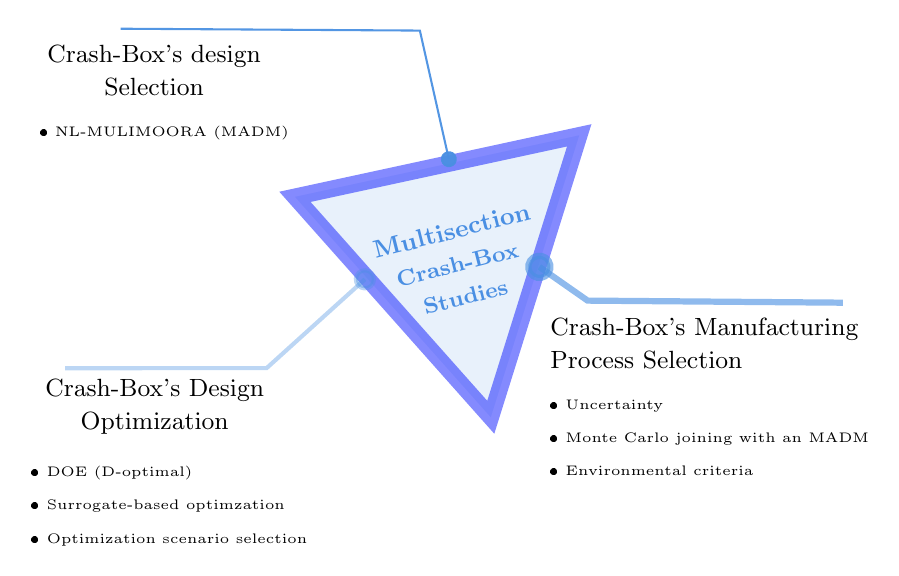
\begin{tikzpicture}[x=0.75pt,y=0.75pt,yscale=-1,xscale=1]
			%uncomment if require: \path (0,300); %set diagram left start at 0, and has height of 300
			
			%Shape: Triangle [id:dp28985420896111713] 
			\draw  [color={rgb, 255:red, 19; green, 30; blue, 254 }  ,draw opacity=0.52 ][fill={rgb, 255:red, 74; green, 144; blue, 226 }  ,fill opacity=0.13 ][line width=6]  (280.47,80.8) -- (237.85,216.63) -- (143.5,110.43) -- cycle ;
			%Straight Lines [id:da6781629732834764] 
			\draw [color={rgb, 255:red, 74; green, 144; blue, 226 }  ,draw opacity=0.62 ][line width=2.25]    (261.26,144.17) -- (284.5,160.43) -- (407.5,161.43) ;
			\draw [shift={(261.26,144.17)}, rotate = 34.97] [color={rgb, 255:red, 74; green, 144; blue, 226 }  ,draw opacity=0.62 ][fill={rgb, 255:red, 74; green, 144; blue, 226 }  ,fill opacity=0.62 ][line width=2.25]      (0, 0) circle [x radius= 5.36, y radius= 5.36]   ;
			%Straight Lines [id:da3748436050233743] 
			\draw [color={rgb, 255:red, 74; green, 144; blue, 226 }  ,draw opacity=0.95 ][line width=0.75]    (59.5,29.43) -- (203.69,30.33) -- (217.65,92.28) ;
			\draw [shift={(217.65,92.28)}, rotate = 77.3] [color={rgb, 255:red, 74; green, 144; blue, 226 }  ,draw opacity=0.95 ][fill={rgb, 255:red, 74; green, 144; blue, 226 }  ,fill opacity=0.95 ][line width=0.75]      (0, 0) circle [x radius= 3.35, y radius= 3.35]   ;
			%Straight Lines [id:da019947602617983007] 
			\draw [color={rgb, 255:red, 74; green, 144; blue, 226 }  ,draw opacity=0.37 ][line width=1.5]    (177.2,150.18) -- (129.86,192.95) -- (32.83,193) ;
			\draw [shift={(177.2,150.18)}, rotate = 137.9] [color={rgb, 255:red, 74; green, 144; blue, 226 }  ,draw opacity=0.37 ][fill={rgb, 255:red, 74; green, 144; blue, 226 }  ,fill opacity=0.37 ][line width=1.5]      (0, 0) circle [x radius= 4.36, y radius= 4.36]   ;
			
			% Text Node
			\draw (17.98,36.01) node [anchor=north west][inner sep=0.75pt]  [rotate=-359.98] [align=left] {\begin{minipage}[lt]{84.58180000000002pt}\setlength\topsep{0pt}
					\begin{center}
						{\small Crash-Box's design }\\{\small Selection }
					\end{center}
					
			\end{minipage}};
			% Text Node
			\draw (17.25,196.97) node [anchor=north west][inner sep=0.75pt]  [rotate=-359.98] [align=left] {\begin{minipage}[lt]{86.105pt}\setlength\topsep{0pt}
					\begin{center}
						{\small Crash-Box's Design }\\{\small Optimization }
					\end{center}
					
			\end{minipage}};
			% Text Node
			\draw (265.31,167.52) node [anchor=north west][inner sep=0.75pt]  [rotate=-359.98] [align=left] {{\small Crash-Box's Manufacturing }\\{\small Process Selection }};
			% Text Node
			\draw (176.91,123.9) node [anchor=north west][inner sep=0.75pt]  [rotate=-345.77] [align=left] {\begin{minipage}[lt]{56.277072000000004pt}\setlength\topsep{0pt}
					\begin{center}
						\textbf{\textcolor[rgb]{0.29,0.56,0.89}{{\small Multisection}}}\\\textbf{\textcolor[rgb]{0.29,0.56,0.89}{{\footnotesize Crash-Box}}}\\\textbf{\textcolor[rgb]{0.29,0.56,0.89}{{\footnotesize Studies}}}\\
					\end{center}
					
			\end{minipage}};
						\pause
			% Text Node
			\draw (19,75) node [anchor=north west][inner sep=0.75pt]   [align=left] {{\tiny • NL-MULIMOORA (MADM)}};
			% Text Node
			\draw (15,239) node [anchor=north west][inner sep=0.75pt]   [align=left] {{\tiny • DOE (D-optimal)}\\{\tiny • Surrogate-based optimzation}\\{\tiny • Optimization scenario selection}};
			% Text Node
			\draw (265,207) node [anchor=north west][inner sep=0.75pt]   [align=left] {{\tiny • Uncertainty }\\{\tiny • Monte Carlo joining with an MADM}\\{\tiny • Environmental criteria}};
			
			
		\end{tikzpicture}
		
	\end{frame}
	
	
	%% ------------------------------------------------
	\subsection{	 \oldstylenums{2016}-\oldstylenums{2017} ~~~~ {Crash-Box selection (Master's thesis)} }
	%------------------------------------------------
	
	\begin{frame}
		\frametitle{\begin{tabular}{ll}
				\circled{1} & \begin{tabular}{l}
					Master's Thesis: \\ 
					Crash-Box Selection employing \textsc{Madm} \& Simulation \\ 
				\end{tabular} \\ 
		\end{tabular}}
		
		\begin{itemize}{\footnotesize 
				\item {Proposing a hybrid method \textsc{Madm},  \hyperlink{4}{\textsc{Multimoora$ ^{ \Exl} $}}  + \hyperlink{3}{\textsc{Nl$ ^{ \Exl} $}}  $ \Longrightarrow $\textsc{Nl-Multimoora}}   
				\item \hyperlink{5}{Simulating the crashing process$ ^{ \Exl} $}
				\item {Generating, Sorting and Selecting  the best design in two steps:}
				\begin{itemize}	{\scriptsize
						\item \hyperlink{6}{The best design selection through 39 designs based on Length \& Thickness $ ^{ \Exl} $}% (constant taper's Angle) 
						\item  \hyperlink{7}{The best design selection through 16 designs based on Taper's Angle $ ^{ \Exl} $}
					}
				\end{itemize}
				%		\item {Sortig the candidates by \textsc{Nl-Multimoora}}
				%		\item {considering the Taper's Angle}
				\item {The best prototype design selected}	
			}
		\end{itemize}		
		\begin{figure}[h]
			
			\centering
			\includegraphics[width=0.3\linewidth]{2019-06-29_15-34-45}
			\caption{{\tiny Simulation of the conical segmented tube under axial loading (Souzangarzadeh et al. 2017)}}
			\label{fig:2019-06-2915-34-45}
		\end{figure}
		
	\end{frame}
	
		\begin{frame}%{	\circled{4}}
		%{Crash-Box Multi-Objective Optimization \& selection: D-Optimal design, \textsc{Cw-Multimoora} \& Numerical}
\textbf{		Proposed prototype selection process:}\\ 				\pause
		~
		{\footnotesize
			
			\textcolor{blue}{$ \bigtriangledown $} \textbf{Step one}
			\textcolor{blue}{$ \Longrightarrow $} Modeling the crushing process of Aluminum segmented tubes with 3D Solid elements. \\
		%	\textcolor{blue} {$ \Longrightarrow $}  \\~~~ 
						\pause
			~
			\\
			\textcolor{blue}{	$ \bigtriangledown $} \textbf{Step two}
			\textcolor{blue}{$ \Longrightarrow $}  Generating 39 points \textcolor{blue}{$ \Longrightarrow $} 	\textsc{Nl-Multimoora} selected the best design base on thicknesses and lengths  
		 \textcolor{blue}{$ \Longrightarrow $} Specifying the best thicknesses and lengths for the next step \\
		 				\pause
			~
			\\
			\textcolor{blue}	{	$ \bigtriangledown $} \textbf{Step three}
			\textcolor{blue}{$ \Longrightarrow $} Considering different taper angles 
			 \textcolor{blue}{$ \Longrightarrow $}  Generating other 14 points + the two best designs from second step
			\textcolor{blue}{$ \Longrightarrow $} Selecting the best design base on taper angle through 
			\textsc{Nl-Multimoora} 
		}
		
	\end{frame}
	
	
	
	%% ------------------------------------------------
	\subsection{	 \oldstylenums{2017} ~~~~ ~~~~ ~ {Foam-Filled Crash-Box with Initiator} }
	%------------------------------------------------
	
	\begin{frame}{}
		\frametitle{\begin{tabular}{ll}
				\circled{2} & \begin{tabular}{l}
					Foam-Filled Crash-Box with Initiator:  \\ 
					Experimental \& Numerical \\ 
				\end{tabular} \\ 
		\end{tabular}}
		
		{\scriptsize 		\begin{itemize}
				\item Evaluating the effect of Initiator \& foam on the behavior  of the Crash-box
				\begin{itemize}
					{\tiny 	
						\item \hyperlink{8}{Numerically $ ^{ \Exl} $}
						\item \hyperlink{9}{Experimentally $ ^{ \Exl} $} }
				\end{itemize}
				%	{Crushing tests on foam-filled rectangular tubes with and without initiator} 	
				\item Detecting the effect of \hyperlink{8}{the Initiator $ ^{ \Exl} $}
				\item Detecting the most efficient Initiator's length
				
		\end{itemize}}
		
		~
		\\
		~
		\begin{columns}
			\column{.5\linewidth}
			
			\begin{figure}[h]
				\centering
				\includegraphics[width=0.8\linewidth]{2019-06-28_19-07-50}
				
				\label{fig:2019-06-2819-07-50}
			\end{figure}
			\column{.5\linewidth}
			
			\begin{figure}[h]
				\centering
				\includegraphics[width=0.8\linewidth]{2019-06-28_19-07-06}
				
				\label{fig:2019-06-2819-07-06}
			\end{figure}
			
		\end{columns}
		\begin{center}
			{\tiny Different stages of crushing for partially foam-filled with an initiator (Razazan et al. 2018)}
		\end{center}
	\end{frame}
	
	%% ------------------------------------------------
	
	
	\subsection{	 \oldstylenums{2018} ~~~~ ~~~~ ~ {Inversion of Crash-Box  Process} }
	
	\begin{frame}{}
		\frametitle{\begin{tabular}{ll}
				\circled{3} & \begin{tabular}{l}
					Inversion of Crash-Box  Process:   \\ 
					Experimental \& Numerical \\ 
				\end{tabular} \\ 
		\end{tabular}}
		{\scriptsize 		\begin{itemize}
				\item Evaluating the effect of triggering, foam \& inversion process on the behavior  of the Crash-box
				\begin{itemize}
				{\tiny 	
					\item \hyperlink{10}{Numerically $ ^{ \Exl} $}
					\item \hyperlink{11}{Experimentally $ ^{ \Exl} $} }
			\end{itemize}
	 \item Detecting the effect of \hyperlink{11}{the inversion mechanism, $ ^{ \Exl} $}
	%	\item Comparing the external and internal inversion mechanism
				%	{Crushing tests on foam-filled rectangular tubes with and without initiator} 	
				%	\item Detecting the most efficient initiator's length
				%	{Modelling the Crash-Boxes' Crushing}
				
		\end{itemize}}
		
		~\\
		
		\begin{columns}
			\column{.5\linewidth}
			\begin{figure}[h]
				\centering
				\includegraphics[width=0.8\linewidth]{2019-06-29_12-44-44}
				
				\label{fig:2019-06-2912-44-44}
			\end{figure}
			
			\column{.5\linewidth}
			\begin{figure}[h]
				\centering
				\includegraphics[width=0.8\linewidth]{2019-06-29_12-45-04}
				\label{fig:2019-06-2912-45-04}
			\end{figure}
		\end{columns}
		\begin{center}
			{\tiny Crushed shapes of empty and foam-filled circular specimens derived from experimental and numerical simulation (Rezvani and Souzangarzadeh 2020)}
		\end{center}
	\end{frame}
	%% ------------------------------------------------------------------------------------------------------
		\subsection{	 \oldstylenums{2024} ~~~~ ~~~~ ~ {End‑capped multi‑segmented conical foam filled-tubes} }
	% -------------------------------------------------------------------------------------------------------
	\begin{frame}{}
		\frametitle{\begin{tabular}{ll}
				\circled{4} & \begin{tabular}{l}
					End‑capped multi‑segmented conical foam filled-tubes:   \\ 
					Experimental \& Numerical \\ 
				\end{tabular} \\ 
		\end{tabular}}
		{\scriptsize 	
				\begin{itemize}
				\item Evaluating the effect of End‑capped multi‑segmented conical foam filled-tubes under under axial and oblique loads
				\begin{itemize}
					{\tiny 	
						\item {Numerically }
						\item {Experimentally}}
				\end{itemize}
				\item Detecting the effect of 	End‑capping and Foam,
				%	\item Comparing the external and internal inversion mechanism
				%	{Crushing tests on foam-filled rectangular tubes with and without initiator} 	
				%	\item Detecting the most efficient initiator's length
				%	{Modelling the Crash-Boxes' Crushing}
				
		\end{itemize}}
		
		~\\
		
		\begin{columns}
			\column{.5\linewidth}
			\begin{figure}[h]
				\centering
				\includegraphics[width=0.8\linewidth]{Screenshot2024-11-18200720}
				
				\label{fig:2024-11-18200720}
			\end{figure}

		\column{.5\linewidth}
			\begin{figure}[h]
				\centering
				\includegraphics[width=0.8\linewidth]{2024-11-18201220}
			\label{fig:2024-11-18201220}
			\end{figure}
		\end{columns}
		\begin{center}
			{\tiny Performance of end‑capped multi‑segmented conical tubes filled with foam under axial and oblique loads as an energy absorber (Rezvani and Souzangarzadeh 2024)}
		\end{center}
	\end{frame}
	%% ------------------------------------------------------------------------------------------------------
	\subsection{	 \oldstylenums{2018}-\oldstylenums{2019} ~~~~ {Crash-Box Multi-Objective Optimization }}
	%------------------------------------------------
	
	\begin{frame}
		\frametitle{\begin{tabular}{ll}
				\circled{5} & \begin{tabular}{l}
					Crash-Box Multi-Objective Optimization \& selection:\\ D-Optimal design, \textsc{Cw-Multimoora} \& Numerical \\ 
				\end{tabular} \\ 
		\end{tabular}}
		
		
		{~~\\ Optimization the design of Crash-box employing \textsc{Doe}, \textsc{Madm}, \& {Simulation} }
		\\
		{\scriptsize
			$ \triangleright $ \hyperlink{12}{Five design variables \& Ten Objective Functions $ ^{ \Exl} $} }
		
		
		\begin{columns}
			\column{.5\linewidth}
			\begin{figure}[h]
				\centering
				\includegraphics	[width=0.6\textwidth]{20.png}
			\end{figure}
			
			\column{.5\linewidth}
			\begin{figure}[h]
				\centering
				\includegraphics[width=0.5\linewidth]{"D:/ARTICLES/Optimization of cylindrical segmented/springer/images/crushing"}
			\end{figure}
		\end{columns}
		\begin{center}
			{\tiny Deforming process of the selected tube under  axial,  15$^\circ$, and 30$^\circ$ loads (Souzangarzadeh et sl. 2020)}
		\end{center}
	\end{frame}
	
	\begin{frame}%{	\circled{4}}
		%{Crash-Box Multi-Objective Optimization \& selection: D-Optimal design, \textsc{Cw-Multimoora} \& Numerical}
		\textbf{Proposed optimization and selection process:}\\
		~				\pause
		{\footnotesize
			
			\textcolor{blue}{$ \bigtriangledown $} \hyperlink{13}{DoE (RSM  D-optimal)$ ^{ \Exl} $}  \textcolor{blue}{$ \Longrightarrow $} 34 points \textcolor{blue} {$ \Longrightarrow $} Ten regression models \\~~~ \textcolor{blue} {$ \Longrightarrow $} Comparing the regression model with FEM \\~~~
			\textcolor{blue}	{$ \Longrightarrow $} Adding more points to improve the regression models.\\				\pause
			~
			\\
			\textcolor{blue}{	$ \bigtriangledown $} 16 optimization scenarios \textcolor{blue}{$ \Longrightarrow $}  \hyperlink{14}{16 optimized designs $ ^{ \Exl} $}\\					\pause
			~
			\\			
			\textcolor{blue}	{	$ \bigtriangledown $} 
			\hyperlink{15}{Using  combinative weighting (CW) method to combine three differnt methods $ ^{ \Exl} $} 	\\			\pause
			~
			\\			
			\textcolor{blue}	{	$ \bigtriangledown $} \hyperlink{16}{Selecting the best  candidate/scenarios through \textsc{Cw-Multimoora}$ ^{ \Exl} $ }
		}
		
	\end{frame}
	
	
	%% -------------------------------------------------------------------------------------
	
	\subsection{	 \oldstylenums{2019}-\oldstylenums{2022} ~~~~ Crash-Box Manufacturing Process Selection}
	
	%------------------------------------------------
	%		\begin{frame}
	
	%	$ \looparrowright $ ~~~~~~~~	Crash-Box Manufacturing Process Selection
	%      \end{frame}
	\begin{frame}\frametitle{{Automobile Crash-Box Manufacturing Process Selection}}
		
		\frametitle{\begin{tabular}{ll}
				$ \circled{6} $ & Automobile Crash-Box Manufacturing Selection \\ 
		\end{tabular}}
		
	%	{Manufacturing Process Selection\\	}
		%\pause
		~
		
		Assumptions and Conditions:\\
		~
		{\scriptsize 	\begin{itemize}
				
				\item Cylindrical-Steel-segmented tube (Souzangarzadeh et al. 2020) and Conical-aluminum-segmented tube (Souzangarzadeh et al. 2017)
				
				\item
				{Uncertain data in the case study location, Iran}
				\item Extracted data of time and cost were interval not exact
					\end{itemize}}
				%from industry~~
				~~
				~~\\				\pause
				Methods:
				\\
				~~~
					{\scriptsize 	\begin{itemize}
				%	{Elimination  the Trial \& error method of problem solving}
				%, common in some Iran's industries}
				\item ELECTRE-IDAT as MADM method deals with interval and exact data
				
				\item Using Monte Carlo to simulate the selection process for 5000 times
				%	{Manufacturing Processes \& materials  alternatives}
				%	\item
				% \capitalisewords{calculating the cost functions of each process (Decision matrix)}
				
				\item 	{The most promising manufacturing processes and material-design  selected}
				
			\end{itemize}
		}
	\end{frame}
	
	%------------------------------------------------
	
	
	
	\begin{frame}
		\frametitle{References}
		\tiny{
			\begin{thebibliography}{99} % Beamer does not support BibTeX so references must be inserted manually as below
				\bibitem rN.N, Hussain, S.P, Regalla,   Y.V.D., Rao,  2017
				\newblock {Comparative study of trigger configuration for enhancement of Crashworthiness of automobile Crash box subjected to axial impact loading. }
				\newblock \emph {Procedia Engineering, 173, pp.1390-1398.}
				
				
				
				\bibitem 4\textbf{H, Souzangarzadeh}, M,	Rezvani, A,	 A,	Jahan, 2017
				\newblock Selection of optimum design for conical segmented aluminum tubes as energy absorbers: Application of MULTIMOORA method
				\newblock \emph{Applied Mathematical Modelling} 
				
				\bibitem 3M, Razazan, M.J, Rezvani,  \textbf{H, Souzangarzadeh},  2018
				\newblock Evaluation of the Performance of Initiator on Energy Absorption of Foam-Filled Rectangular Tubes: Experimental and Numerical Assessment 
				\newblock \emph{Experimental Techniques} 
				
				\bibitem t M.J, Rezvani,  \textbf{H, Souzangarzadeh},  2020
				\newblock Effects of triggering and polyurethane foam on energy absorption of thin-walled circular tubes under the inversion process 
				\newblock \emph{Journal of Energy Storage} 
				
				\bibitem r\textbf{H, Souzangarzadeh}, A,	Jahan, M,	Rezvani, A,	Milani, 2020
				\newblock{Multi-objective optimization of cylindrical segmented tubes as energy absorbers under oblique crushes: D-optimal design and integration ofMULTIMOORA with combinative weighting}
				\newblock \emph {Structural and Multidisciplinary Optimization}
				
	\bibitem rN.A.Z. Abdullah, M.S.M. Sani, M.S. Salwani, N.A. Husain 2020
\newblock {A review on crashworthiness studies of crash box structure}
\newblock \emph{Thin-Walled Structures journal}

\bibitem t
N S B, Yusof,
 S M, Sapuan,
 M T H, Sultan,
 M, Jawaid,
 M A, Maleque,
2017
\newblock {Design and materials development of automotive crash box : a review}
\newblock \emph{Ci{\^{e}}ncia {\&} Tecnologia dos Materiais}
				
			
			\end{thebibliography}
		}
	\end{frame}
	
	%------------------------------------------------
	
	\begin{frame}
		\Huge{\centerline{The End}}
	\end{frame}
	
	%----------------------------------------------------------------------------------------
	
	\appendix
	\begin{frame}{Appendix 1}	
		\hypertarget{1}{}

		\begin{figure}[H]%simples tube plot
			\centering
			\includegraphics[width=0.6\linewidth]{15}
			\caption{\tiny Typical load-displacement curve of the conical segmented tube}\label{nemE}
		\end{figure}
		
		
	\end{frame}
	\begin{frame}{Appendix 2}
				\hypertarget{2}{}
		\tiny
	
		
		\begin{block}{ \scriptsize	\circled{1} Absorbed energy}
			The total  absorbed energy: %, $ E_{absorbed} $: % is equal to the area under the load-displacement curve, where:
			$ \Longrightarrow $
			$ 	E_{absorbed} =\int Fd\delta $
			
			Where  $F$ and $\delta$ are the crush force and crush distance, respectively.
		\end{block}
		\begin{block}{ \scriptsize	\circled{2} Mean crushing load}
			%As one of the most important parameters affecting the  behavior of tubes under axial load, mean crushing load ($F_{m}$) is equal to 
			The ratio of total absorbed energy to total crushing distance.
			$ \Longrightarrow $
			$ 	F_{m} =\frac{1}{\delta_{t}}\int Fd\delta $
			
		\end{block}
		\begin{block}{ \scriptsize	\circled{3} Maximum crushing load }
			%According to Fig.~\ref{nemE}, 
			The initial peak load ($F_{i}$) occurs at the onset of the curve. 
			The maximum peak load ($F_{Max}$) in conical segmented tubes usually occurs at the end of the crush range%before densification. It is desirable to find an optimum energy absorber design that has the highest amount of absorbed energy and the lowest $F_{i}$ and $F_{Max}$, while it has a light weight. 
		\end{block}
		\begin{block}{ \scriptsize	\circled{4} Crush force efficiency (CFE)}
			This parameter is used to compare the efficiency of different energy absorbers.% It is equal to the ratio of mean crushing load to the maximum crushing load~\cite{Rezvani2015}.  
			$ \Longrightarrow $
			$ 	CFE=\dfrac{F_{m}}{F_{Max}}  $
			
		\end{block}
			\begin{block}{\scriptsize	\circled{5} The specific energy absorption} Energy Absorbed Per Unit Mass
			$ \Longrightarrow $
			$SEA =  \frac {E_{absorbed}}{M} $
		\end{block}
		
	\end{frame}
	
	
	
	\begin{frame}{Appendix 3}
				\hypertarget{3}{}
				\begin{block}{	NL 	$ \Longrightarrow $	subjective weighting method 	$ \Longrightarrow $ any numeric weight between 0 and 1 for each criteria:}
\begin{center}
	$	W_{j,NL}=\frac{\sum_{k=1}^{n}C_{jk} }{\sum_{j=1}^{n}\sum_{k=1}^{n}C_{jk}}, j \hspace{0.1cm} and \hspace{0.1cm} k=\{1,...,n\}\hspace{0.1cm} and \hspace{0.1cm}j\neq k$
\end{center}
				\end{block}


	
	\begin{figure}
		\centering
		\includegraphics[width=0.7\linewidth]{20.jpg}
		\caption{}
		\label{fig:20}
	\end{figure}
	\end{frame}
	
	
	
	\begin{frame}{}
				\hypertarget{4}{}
		\tiny
		\begin{block}{The ratio system}
				Normalized matrix multiplied by the deviation of the subjective weight of beneficial attributes from the non-beneficial ones, where \emph{g} is the number of beneficial attributes, and \emph{n}  is the number of all attributes:
			
			
			
			$ 	y^{w}_{i}=\sum_{j=1}^{g}  w_{j} {x^{*}_{ij}}-\sum_{j=g+1}^{n} w_{j} x^{*}_{ij} $
			
			Based on the ratio system, the optimum alternative  has the maximum assessment value of $y^{w}_{i}$.
		
			
		\end{block}
	
	\begin{block}{The reference point approach}
the maximal attribute reference point vector (r) and the deviation of normalized rating from the reference point (d).


$ 	r_{j}= \left\{
	\begin{aligned}
		\max_{i}~x^{*}_{ij}, ~~~& j \leq g,\\
		\min_{i}~x^{*}_{ij}, ~~~& j > g.
	\end{aligned} \right.
 $
~~~~~~~~~~$ \Longrightarrow $ ~~~~~~~~
$ 	d_{ij}=(r_{j}-x^{*}_{ij}) $
~~~~~~~~~~$ \Longrightarrow $ ~~~~~~~~~
$ 	z^{w}_{i} =\max_{j}~w_{j}d_{ij} $


Based on the reference point approach, the optimum alternative has the minimum assessment value of $ z^{w}_{i} $%~\cite{Datta2013}:

	\end{block}

\begin{block}{The full multiplicative form}
	The value of the full multiplicative form, which was weighted by considering the subjective weight as the exponent:

$ 	{U}^{w}_{i}=\frac{\prod_{j=1}^{g}(x_{ij}^{*})^{w_{j}}}{\prod_{j=g+1}^{n}(x_{ij}^{*})^{w_{j}}} $


the optimum alternative  has the maximum assessment value of ${U}^{w}_{i}$.

\end{block}

\begin{block}{Final rank}
	
The subordinate ranks calculated above can be conjoined to the final rank, which is known as the MULTIMOORA rank, by utilizing the dominance theory.
\end{block}
	\end{frame}       

\begin{frame}{Appendix 5}
		\hypertarget{5}{}
\begin{figure}
	\centering
	\includegraphics[width=0.4\linewidth]{25}
%	\caption{Simulation of crushing process}
	\label{fig:25}
\end{figure}	

\end{frame}

\begin{frame}	\hypertarget{6}{}
	\begin{figure}
		\centering
		\includegraphics[width=0.55\linewidth]{19}
		\caption{}
	%	\label{fig:20}
	\end{figure}
 \end{frame}
\begin{frame}{Appendix 7}	\hypertarget{7}{}
	\begin{figure}
		\centering
		\includegraphics[width=0.65\linewidth]{24}
		\caption{}
		%	\label{fig:20}
	\end{figure}
\end{frame}
%----------------------------------------------------------------------------------------
 \begin{frame}{Appendix 8}
 		\hypertarget{8}{}
 	
 	\begin{columns}

 	\column{.45\textwidth}
	\begin{figure}
		\centering
		\includegraphics[width=0.8\linewidth]{16}
		\caption{}
		%	\label{fig:17}
	\end{figure}
	\column{.45\textwidth}
	\begin{figure}
		\centering
		\includegraphics[width=0.8\linewidth]{17}
		\caption{}
		\label{fig:17}
	\end{figure}
	\end{columns}
\end{frame}
	
\begin{frame}\hypertarget{9}{}
\begin{columns}
	\column{.45\textwidth}
	\begin{figure}
		\centering
		\includegraphics[width=0.65\linewidth]{175}
		%	\caption{}
		%	\label{fig:17}
	\end{figure}
	\column{.49\textwidth}
	\begin{figure}
		\centering
		\includegraphics[width=0.7\linewidth]{165}
		%	\caption{}
		%	\label{fig:16}
	\end{figure}
\end{columns}
\end{frame}

\begin{frame}{{Appendix 10}}\hypertarget{10}{}

\begin{figure}
	\centering
	\includegraphics[width=0.5\linewidth]{50}

		\includegraphics[width=0.65\linewidth]{51}
	\caption{}
%	\label{fig:51}
\end{figure}
\begin{figure}
	\centering

	\caption{}
	\label{fig:51}
\end{figure}
\end{frame}


%----------------------------------------------------------------------------------
\begin{frame}\hypertarget{11}{}
	\begin{figure}
		\centering
		\includegraphics[width=0.4\linewidth]{52}
		\caption{}
		%	\label{fig:51}
	\end{figure}
\begin{columns}
	\column{.45\textwidth}
	\begin{figure}
		\centering
		\includegraphics[width=0.6\linewidth]{54}
		\caption{}
		%		\label{fig:51}
	\end{figure}
	\column{.49\textwidth}
	\begin{figure}
		\centering
		\includegraphics[width=0.45\linewidth]{53}
		\caption{}
%		\label{fig:51}
	\end{figure}
\end{columns}
	\end{frame}
%----------------------------------------------------------------------------------
\begin{frame}\hypertarget{12}{}
	\begin{figure}
		\centering
		\includegraphics[width=0.45\linewidth]{3}
		\caption{}
		%		\label{fig:51}
	\end{figure}
	\begin{columns}
		\column{.45\textwidth}
		\begin{figure}
			\centering
			\includegraphics[width=0.65\linewidth]{1}
			%	\caption{}
			%	\label{fig:17}
		\end{figure}
		\column{.45\textwidth}
		\begin{figure}
			\centering
			\includegraphics[width=0.5\linewidth]{2}
			%	\caption{}
			%	\label{fig:16}
		\end{figure}
	\end{columns}
\end{frame}

%---------------------------------------------------------------------------------
\begin{frame}{Appendix 13}\hypertarget{13}{}
	
\begin{figure}
	\centering
	\includegraphics[width=0.7\linewidth]{6}
	\caption{}
	\label{fig:6}
\end{figure}
\end{frame}
%----------------------------------------------------------------------------------
\begin{frame}{Appendix 14} \hypertarget{14}{}
	
\begin{figure}
	\centering
	\includegraphics[width=0.7\linewidth]{5}
	\caption{}
	\label{fig:5}
\end{figure}
\end{frame}
%----------------------------------------------------------------------------------

\begin{frame}{Appendix 15} \hypertarget{15}{}
	
	\begin{figure}
		\centering
		\includegraphics[width=0.7\linewidth]{9}
		\caption{}
		\label{fig:5}
	\end{figure}
\end{frame}

\begin{frame} {Appendix 16}\hypertarget{16}{}
	
	\begin{figure}
		\centering
		\includegraphics[width=0.7\linewidth]{12}
		\caption{}
		\label{fig:5}
	\end{figure}
\end{frame}


\end{document} 
%----------------------------------------------------------------------------------------
%----------------------------------------------------------------------------------------
%----------------------------------------------------------------------------------------
%----------------------------------------------------------------------------------------
%----------------------------------------------------------------------------------------
%----------------------------------------------------------------------------------------
%----------------------------------------------------------------------------------------\\
%----------------------------------------------------------------------------------------
%----------------------------------------------------------------------------------------
%----------------------------------------------------------------------------------------\\
%----------------------------------------------------------------------------------------\\
%----------------------------------------------------------------------------------------\\
%----------------------------------------------------------------------------------------\\
%----------------------------------------------------------------------------------------\\
%----------------------------------------------------------------------------------------\\
%----------------------------------------------------------------------------------------\\
